\PassOptionsToPackage{unicode=true}{hyperref} % options for packages loaded elsewhere
\PassOptionsToPackage{hyphens}{url}
%
\documentclass[]{article}
\usepackage{lmodern}
\usepackage{amssymb,amsmath}
\usepackage{ifxetex,ifluatex}
\usepackage{fixltx2e} % provides \textsubscript
\ifnum 0\ifxetex 1\fi\ifluatex 1\fi=0 % if pdftex
  \usepackage[T1]{fontenc}
  \usepackage[utf8]{inputenc}
  \usepackage{textcomp} % provides euro and other symbols
\else % if luatex or xelatex
  \usepackage{unicode-math}
  \defaultfontfeatures{Ligatures=TeX,Scale=MatchLowercase}
\fi
% use upquote if available, for straight quotes in verbatim environments
\IfFileExists{upquote.sty}{\usepackage{upquote}}{}
% use microtype if available
\IfFileExists{microtype.sty}{%
\usepackage[]{microtype}
\UseMicrotypeSet[protrusion]{basicmath} % disable protrusion for tt fonts
}{}
\IfFileExists{parskip.sty}{%
\usepackage{parskip}
}{% else
\setlength{\parindent}{0pt}
\setlength{\parskip}{6pt plus 2pt minus 1pt}
}
\usepackage{hyperref}
\hypersetup{
            pdftitle={Flujo de análisis en clasificación supervisada},
            pdfauthor={Laura Rodríguez Navas},
            pdfborder={0 0 0},
            breaklinks=true}
\urlstyle{same}  % don't use monospace font for urls
\usepackage[margin=1in]{geometry}
\usepackage{color}
\usepackage{fancyvrb}
\newcommand{\VerbBar}{|}
\newcommand{\VERB}{\Verb[commandchars=\\\{\}]}
\DefineVerbatimEnvironment{Highlighting}{Verbatim}{commandchars=\\\{\}}
% Add ',fontsize=\small' for more characters per line
\usepackage{framed}
\definecolor{shadecolor}{RGB}{248,248,248}
\newenvironment{Shaded}{\begin{snugshade}}{\end{snugshade}}
\newcommand{\AlertTok}[1]{\textcolor[rgb]{0.94,0.16,0.16}{#1}}
\newcommand{\AnnotationTok}[1]{\textcolor[rgb]{0.56,0.35,0.01}{\textbf{\textit{#1}}}}
\newcommand{\AttributeTok}[1]{\textcolor[rgb]{0.77,0.63,0.00}{#1}}
\newcommand{\BaseNTok}[1]{\textcolor[rgb]{0.00,0.00,0.81}{#1}}
\newcommand{\BuiltInTok}[1]{#1}
\newcommand{\CharTok}[1]{\textcolor[rgb]{0.31,0.60,0.02}{#1}}
\newcommand{\CommentTok}[1]{\textcolor[rgb]{0.56,0.35,0.01}{\textit{#1}}}
\newcommand{\CommentVarTok}[1]{\textcolor[rgb]{0.56,0.35,0.01}{\textbf{\textit{#1}}}}
\newcommand{\ConstantTok}[1]{\textcolor[rgb]{0.00,0.00,0.00}{#1}}
\newcommand{\ControlFlowTok}[1]{\textcolor[rgb]{0.13,0.29,0.53}{\textbf{#1}}}
\newcommand{\DataTypeTok}[1]{\textcolor[rgb]{0.13,0.29,0.53}{#1}}
\newcommand{\DecValTok}[1]{\textcolor[rgb]{0.00,0.00,0.81}{#1}}
\newcommand{\DocumentationTok}[1]{\textcolor[rgb]{0.56,0.35,0.01}{\textbf{\textit{#1}}}}
\newcommand{\ErrorTok}[1]{\textcolor[rgb]{0.64,0.00,0.00}{\textbf{#1}}}
\newcommand{\ExtensionTok}[1]{#1}
\newcommand{\FloatTok}[1]{\textcolor[rgb]{0.00,0.00,0.81}{#1}}
\newcommand{\FunctionTok}[1]{\textcolor[rgb]{0.00,0.00,0.00}{#1}}
\newcommand{\ImportTok}[1]{#1}
\newcommand{\InformationTok}[1]{\textcolor[rgb]{0.56,0.35,0.01}{\textbf{\textit{#1}}}}
\newcommand{\KeywordTok}[1]{\textcolor[rgb]{0.13,0.29,0.53}{\textbf{#1}}}
\newcommand{\NormalTok}[1]{#1}
\newcommand{\OperatorTok}[1]{\textcolor[rgb]{0.81,0.36,0.00}{\textbf{#1}}}
\newcommand{\OtherTok}[1]{\textcolor[rgb]{0.56,0.35,0.01}{#1}}
\newcommand{\PreprocessorTok}[1]{\textcolor[rgb]{0.56,0.35,0.01}{\textit{#1}}}
\newcommand{\RegionMarkerTok}[1]{#1}
\newcommand{\SpecialCharTok}[1]{\textcolor[rgb]{0.00,0.00,0.00}{#1}}
\newcommand{\SpecialStringTok}[1]{\textcolor[rgb]{0.31,0.60,0.02}{#1}}
\newcommand{\StringTok}[1]{\textcolor[rgb]{0.31,0.60,0.02}{#1}}
\newcommand{\VariableTok}[1]{\textcolor[rgb]{0.00,0.00,0.00}{#1}}
\newcommand{\VerbatimStringTok}[1]{\textcolor[rgb]{0.31,0.60,0.02}{#1}}
\newcommand{\WarningTok}[1]{\textcolor[rgb]{0.56,0.35,0.01}{\textbf{\textit{#1}}}}
\usepackage{graphicx,grffile}
\makeatletter
\def\maxwidth{\ifdim\Gin@nat@width>\linewidth\linewidth\else\Gin@nat@width\fi}
\def\maxheight{\ifdim\Gin@nat@height>\textheight\textheight\else\Gin@nat@height\fi}
\makeatother
% Scale images if necessary, so that they will not overflow the page
% margins by default, and it is still possible to overwrite the defaults
% using explicit options in \includegraphics[width, height, ...]{}
\setkeys{Gin}{width=\maxwidth,height=\maxheight,keepaspectratio}
\setlength{\emergencystretch}{3em}  % prevent overfull lines
\providecommand{\tightlist}{%
  \setlength{\itemsep}{0pt}\setlength{\parskip}{0pt}}
\setcounter{secnumdepth}{0}
% Redefines (sub)paragraphs to behave more like sections
\ifx\paragraph\undefined\else
\let\oldparagraph\paragraph
\renewcommand{\paragraph}[1]{\oldparagraph{#1}\mbox{}}
\fi
\ifx\subparagraph\undefined\else
\let\oldsubparagraph\subparagraph
\renewcommand{\subparagraph}[1]{\oldsubparagraph{#1}\mbox{}}
\fi

% set default figure placement to htbp
\makeatletter
\def\fps@figure{htbp}
\makeatother

\usepackage{etoolbox}
\makeatletter
\providecommand{\subtitle}[1]{% add subtitle to \maketitle
  \apptocmd{\@title}{\par {\large #1 \par}}{}{}
}
\makeatother

\title{Flujo de análisis en clasificación supervisada}
\providecommand{\subtitle}[1]{}
\subtitle{Métodos supervisados}
\author{Laura Rodríguez Navas}
\date{Septiembre 2020}

\begin{document}
\maketitle

{
\setcounter{tocdepth}{2}
\tableofcontents
}
\newpage

Empezamos por cargar a nuestro espacio de trabajo los paquetes que
usaremos:

\begin{itemize}
\tightlist
\item
  \textbf{tidyverse}, engloba otros paquetes (\textbf{dplyr},
  \textbf{tidyr}, \textbf{ggplot}, etc.) que facilitan en gran medida el
  análisis exploratorio de los datos.
\item
  \textbf{tm}, específico para minería de textos.
\item
  \textbf{irlba}, específico para \emph{Descomposición de Valores
  Singulares (SVD)} de matrices enormes.
\item
  \textbf{caret}, para realizar tareas de clasificación y regresión.
\item
  \textbf{doParallel}, proporciona computación paralela.
\item
  \textbf{syuzhet}, específico para la extracción de sentimientos de
  textos.
\item
  \textbf{ggcorrplot}, muestra visualizaciones gráficas de matrices de
  correlación usando \emph{ggplot2}.
\end{itemize}

\begin{Shaded}
\begin{Highlighting}[]
\KeywordTok{library}\NormalTok{(tidyverse)}
\KeywordTok{library}\NormalTok{(tm)}
\KeywordTok{library}\NormalTok{(irlba)}
\KeywordTok{library}\NormalTok{(caret)}
\KeywordTok{library}\NormalTok{(doParallel)}
\KeywordTok{library}\NormalTok{(syuzhet)}
\KeywordTok{library}\NormalTok{(ggcorrplot)}
\end{Highlighting}
\end{Shaded}

\hypertarget{anuxe1lisis-exploratorio-de-los-datos}{%
\section{Análisis Exploratorio de los
Datos}\label{anuxe1lisis-exploratorio-de-los-datos}}

Antes de entrenar un modelo predictivo, o incluso antes de realizar
cualquier cálculo con un nuevo conjunto de datos, es muy importante
realizar una exploración descriptiva de los datos. Este proceso nos
permite entender mejor que información contienen cada variable, detectar
posibles errores, etc. además, puede dar pistas sobre qué variables no
son adecuadas para predecir un modelo.

Acorde a la realización del ejercicio propuesto se ha elegido la
competición en Kaggle: \textbf{Real or Not? NLP with Disaster Tweets}.
El dataset de la competición se puede encontrar en el siguiente enlace:
\url{https://www.kaggle.com/c/nlp-getting-started/data}. Este dataset,
con 10.876 instancias, contiene 4 variables explicativas: \textbf{id},
\textbf{keyword}, \textbf{location} y \textbf{text}, y dos valores en la
variable clase \textbf{target} (0 y 1). Como podemos observar la
variable clase es binaria, así que, durante este ejercicio vamos a
aprender un modelo de \emph{clasificación binaria}. El objetivo de este
modelo será predecir si dado un tweet, éste trata sobre un desastre real
o no. Si un tweet trata sobre un desastre real, se predice un 1. Si no,
se predice un 0.

\emph{La clasificación binaria es un tipo de clasificación en el que tan
solo se pueden asignar dos clases diferentes (0 o 1).}

La métrica de evaluación esperada por la competición es \textbf{F1
score}. Para ver como se calcula consultar el siguiente enlace:
\url{https://www.kaggle.com/c/nlp-getting-started/overview/evaluation}.

La partición inicial train-test, no se tiene que realizar, ya que las
instancias de train y test ya vienen definidas en el dataset de la
competición (descargar a nuestro espacio de trabajo los ficheros
\textbf{train.csv} y \textbf{test.csv} de
\url{https://www.kaggle.com/c/nlp-getting-started/data}).

Cargamos a nuestro espacio de trabajo los conjuntos de datos de train y
test descargados, renombrando los valores perdidos como \textbf{NA} para
que los podamos tratar más adelante. También mostramos las dimensiones
de los conjuntos de datos usando la función \textbf{dim}.

\begin{Shaded}
\begin{Highlighting}[]
\NormalTok{train <-}\StringTok{ }\KeywordTok{read.csv}\NormalTok{(}\StringTok{"train.csv"}\NormalTok{, }\DataTypeTok{na.strings=}\KeywordTok{c}\NormalTok{(}\StringTok{""}\NormalTok{, }\StringTok{"NA"}\NormalTok{))}
\NormalTok{test <-}\StringTok{ }\KeywordTok{read.csv}\NormalTok{(}\StringTok{"test.csv"}\NormalTok{, }\DataTypeTok{na.strings=}\KeywordTok{c}\NormalTok{(}\StringTok{""}\NormalTok{, }\StringTok{"NA"}\NormalTok{))}
\KeywordTok{dim}\NormalTok{(train)}
\end{Highlighting}
\end{Shaded}

\begin{verbatim}
## [1] 7613    5
\end{verbatim}

\begin{Shaded}
\begin{Highlighting}[]
\KeywordTok{dim}\NormalTok{(test)}
\end{Highlighting}
\end{Shaded}

\begin{verbatim}
## [1] 3263    4
\end{verbatim}

Vemos que el conjunto de datos de train contiene 7613 instancias y el
conjunto de datos de test contiene 3263 instancias. Cada instancia
contiene las siguientes variables:

\begin{itemize}
\tightlist
\item
  \textbf{id}: un identificador único para cada tweet.
\item
  \textbf{keyword}: una palabra clave del tweet.
\item
  \textbf{location}: la ubicación desde la que se envió el tweet.
\item
  \textbf{text}: el texto del tweet.
\item
  \textbf{target}: solo en el conjunto de datos de train porqué es la
  variable clase a predecir. Indica si un tweet corresponde a un
  desastre real (1) o no (0).
\end{itemize}

\begin{verbatim}
## 'data.frame':    7613 obs. of  5 variables:
##  $ id      : int  1 4 5 6 7 8 10 13 14 15 ...
##  $ keyword : chr  NA NA NA NA ...
##  $ location: chr  NA NA NA NA ...
##  $ text    : chr  "Our Deeds are the Reason of this #earthquake May ALLAH Forgive "..
##  $ target  : int  1 1 1 1 1 1 1 1 1 1 ...
\end{verbatim}

\begin{verbatim}
## 'data.frame':    3263 obs. of  4 variables:
##  $ id      : int  0 2 3 9 11 12 21 22 27 29 ...
##  $ keyword : chr  NA NA NA NA ...
##  $ location: chr  NA NA NA NA ...
##  $ text    : chr  "Just happened a terrible car crash" "Heard about #earthquake is"..
\end{verbatim}

\hypertarget{variable-target}{%
\subsection{\texorpdfstring{Variable
\emph{target}}{Variable target}}\label{variable-target}}

Como ya hemos comentado, la variable \textbf{target} es la variable a
predecir. Es de tipo cuantitativa (de tipo entero) y conviene
convertirla a variable cualitativa, almacenarla con el tipo
\emph{factor}. Para evitar errores, se recodifica para que sus dos
posibles valores sean ``Yes''-``No'' y se convierte a \emph{factor}.

\begin{Shaded}
\begin{Highlighting}[]
\NormalTok{train}\OperatorTok{$}\NormalTok{target <-}\StringTok{ }\KeywordTok{as.factor}\NormalTok{(}\KeywordTok{ifelse}\NormalTok{(train}\OperatorTok{$}\NormalTok{target }\OperatorTok{==}\StringTok{ }\DecValTok{0}\NormalTok{, }\StringTok{"No"}\NormalTok{, }\StringTok{"Yes"}\NormalTok{))}
\KeywordTok{ggplot}\NormalTok{(train, }\KeywordTok{aes}\NormalTok{(}\DataTypeTok{x=}\NormalTok{target)) }\OperatorTok{+}\StringTok{ }\KeywordTok{geom_bar}\NormalTok{(}\KeywordTok{aes}\NormalTok{(}\DataTypeTok{fill=}\NormalTok{target))}
\end{Highlighting}
\end{Shaded}

\begin{center}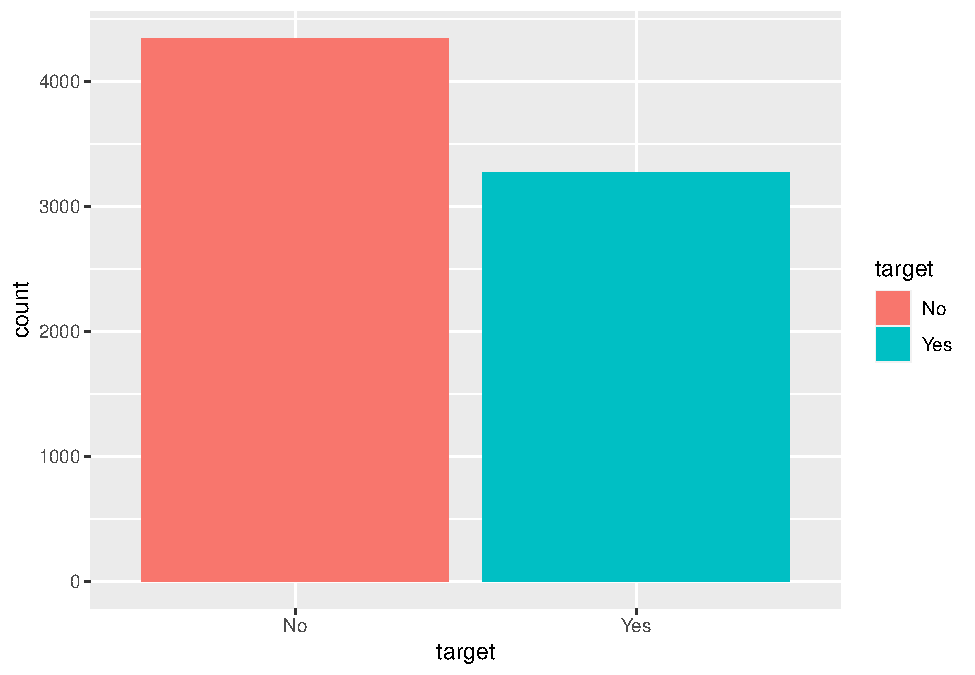
\includegraphics[width=0.7\linewidth]{exercise_files/figure-latex/unnamed-chunk-4-1} \end{center}

Cuando se crea un modelo, es muy importante estudiar la distribución de
la variable clase, ya que, a fin de cuentas, es lo que nos interesa
predecir.

Gráficamente observamos que la distribución de la variable a predecir no
está muy sesgada y está relativamente equilibrada. Hay menos tweets que
se refieren a desastres reales. Además, parece que no presenta un
problema notable de \emph{desbalanceo de clase}, porqué contamos con
muchas observaciones del caso minoritario.

\begin{Shaded}
\begin{Highlighting}[]
\KeywordTok{sum}\NormalTok{(train}\OperatorTok{$}\NormalTok{target }\OperatorTok{==}\StringTok{ "Yes"}\NormalTok{) }\OperatorTok{/}\StringTok{ }\KeywordTok{dim}\NormalTok{(train)[}\DecValTok{1}\NormalTok{] }\OperatorTok{*}\StringTok{ }\DecValTok{100}
\end{Highlighting}
\end{Shaded}

\begin{verbatim}
## [1] 42.96598
\end{verbatim}

\begin{Shaded}
\begin{Highlighting}[]
\KeywordTok{sum}\NormalTok{(train}\OperatorTok{$}\NormalTok{target }\OperatorTok{==}\StringTok{ "No"}\NormalTok{) }\OperatorTok{/}\StringTok{ }\KeywordTok{dim}\NormalTok{(train)[}\DecValTok{1}\NormalTok{] }\OperatorTok{*}\StringTok{ }\DecValTok{100}
\end{Highlighting}
\end{Shaded}

\begin{verbatim}
## [1] 57.03402
\end{verbatim}

Para que un modelo predictivo nos sea útil tendremos que intentar
superar el porcentaje mínimo dado que aproximadamente el 57\% de los
tweets no representan un desastre real (este porcentaje se recalculará
únicamente con el conjunto de datos de train).

Como el objetivo del ejercicio es predecir que tweets pertenecen o no a
un desastre real, el análisis que haremos a continuación se hace realiza
de cada variable explicativa con relación a la variable a predecir
\textbf{target}. Analizando de esta forma, se pueden extraer ideas sobre
que variables están más relacionadas con los desastres reales.

\hypertarget{variable-keyword}{%
\subsection{\texorpdfstring{Variable
\emph{keyword}}{Variable keyword}}\label{variable-keyword}}

La variable explicativa \textbf{keyword} representa una palabra clave en
cada tweet. Vemos las 10 primeras del conjunto de datos de train.

\begin{Shaded}
\begin{Highlighting}[]
\NormalTok{train }\OperatorTok\StringTok{ }\KeywordTok{select}\NormalTok{(keyword) }\OperatorTok\StringTok{ }\KeywordTok{unique}\NormalTok{() }\OperatorTok\StringTok{ }\KeywordTok{head}\NormalTok{(}\DecValTok{10}\NormalTok{)}
\end{Highlighting}
\end{Shaded}

\begin{verbatim}
##                 keyword
## 1                  <NA>
## 32               ablaze
## 68             accident
## 103          aftershock
## 137 airplane%20accident
## 172           ambulance
## 210         annihilated
## 244        annihilation
## 273          apocalypse
## 305          armageddon
\end{verbatim}

Nuestro interés en la variable \textbf{keyword} dentro del análisis
exploratorio de los datos es ver si existen correlaciones entre esta y
la variable a predecir \textbf{target}. Para ello, y como estamos
delante un ejercicio de \emph{Procesamiento del Lenguaje Natural}
realizaremos un análisis de sentimientos.

\emph{El análisis de sentimientos es una técnica de
\href{https://en.wikipedia.org/wiki/Machine_learning}{Machine Learning},
basada en el
\href{https://www.kdnuggets.com/2017/02/natural-language-processing-key-terms-explained.html}{Procesado
del Lenguaje Natural}, que pretende obtener información subjetiva de una
serie de textos. Su aplicación es este caso, consiste en resolver si un
tweet es real o no en relación a un desastre.}

En el análisis de sentimientos usamos los paquetes de R:
\textbf{syuzhet}, \textbf{ggcorrplot} y \textbf{doParallel}.

\begin{itemize}
\tightlist
\item
  El paquete \textbf{syuzhet} cuenta con la función
  \textbf{get\_nrc\_sentiment} que calculará la presencia de los
  diferentes sentimientos dado un conjunto de palabras clave. Los
  argumentos de esta función son:

  \begin{itemize}
  \tightlist
  \item
    \textbf{char\_v}. Un vector de caracteres que en este caso contendrá
    todas las palabras clave.
  \item
    \textbf{language}. Define el lenguaje. Como los tweets están en
    inglés, el lenguaje será el inglés.
  \item
    \textbf{cl}. Para el análisis en paralelo. Es opcional, pero en este
    caso lo usaremos porqué hay muchas palabras clave.
  \end{itemize}
\item
  El paquete \textbf{doParallel} cuenta con las funciones:

  \begin{itemize}
  \tightlist
  \item
    \textbf{makePSOCKcluster}. Crea un clúster de sockets paralelos.
  \item
    \textbf{registerDoParallel}. Registra el número de \emph{cores} que
    usará el clúster creado.
  \item
    \textbf{stopCluster}. Detiene la computación paralela.
  \end{itemize}
\end{itemize}

La computación paralela la usaremos en muchas de las ejecuciones de este
ejercicio ya que nos encontramos delante de un problema de \emph{alta
dimensionalidad}. Eso es, que la dimensionalidad de nuestros datos es
muy elevada y puede reducir drásticamente la eficiencia de los
algoritmos de clasificación supervisada que entrenaremos.

La reducción de la dimensionalidad que aplicaremos en este ejercicio se
realiza más adelante y se calculará teniendo en cuenta las palabras más
frecuentes de los tweets en conjunto de datos.

El análisis de sentimientos de cada palabra clave, usando la función
\textbf{get\_nrc\_sentiment}, consiste en extraer los sentimientos de
cada palabra clave, guardarlos en un nuevo conjunto de datos
(\emph{emotion.df}), con el que calcularemos (paquete \textbf{cor}) y
visualizaremos la matriz de correlaciones (paquete \textbf{ggcorrplot})
entre las palabras clave con relación a la variable a predecir. Es
importante volver a transformar la variable a predecir para realizar los
cálculos, cuando la variable es cualitativa.

\begin{Shaded}
\begin{Highlighting}[]
\NormalTok{cl <-}\StringTok{ }\KeywordTok{makePSOCKcluster}\NormalTok{(}\DecValTok{4}\NormalTok{, }\DataTypeTok{setup_strategy=}\StringTok{"sequential"}\NormalTok{)}
\KeywordTok{registerDoParallel}\NormalTok{(cl)}

\NormalTok{emotion.df <-}\StringTok{ }\KeywordTok{get_nrc_sentiment}\NormalTok{(}\DataTypeTok{char_v =} \KeywordTok{gsub}\NormalTok{(}\StringTok{"_"}\NormalTok{, }\StringTok{" "}\NormalTok{, train}\OperatorTok{$}\NormalTok{keyword), }
                                \DataTypeTok{language =} \StringTok{"english"}\NormalTok{, }\DataTypeTok{cl=}\NormalTok{cl)}

\NormalTok{emotion.df <-}\StringTok{ }\NormalTok{emotion.df }\OperatorTok\StringTok{ }\KeywordTok{data.frame}\NormalTok{(}\DataTypeTok{target =}\NormalTok{ train}\OperatorTok{$}\NormalTok{target)}

\NormalTok{emotion.df}\OperatorTok{$}\NormalTok{target <-}\StringTok{ }\KeywordTok{as.numeric}\NormalTok{(emotion.df}\OperatorTok{$}\NormalTok{target)}

\KeywordTok{cor}\NormalTok{(emotion.df) }\OperatorTok\StringTok{ }
\StringTok{  }\KeywordTok{ggcorrplot}\NormalTok{(}\DataTypeTok{lab =} \OtherTok{TRUE}\NormalTok{, }
             \DataTypeTok{title =} \StringTok{"Matriz de correlación entre }\CharTok{\textbackslash{}n}\StringTok{keyword y target"}\NormalTok{,}
             \DataTypeTok{legend.title =} \StringTok{"correlation"}\NormalTok{)}
\end{Highlighting}
\end{Shaded}

\begin{center}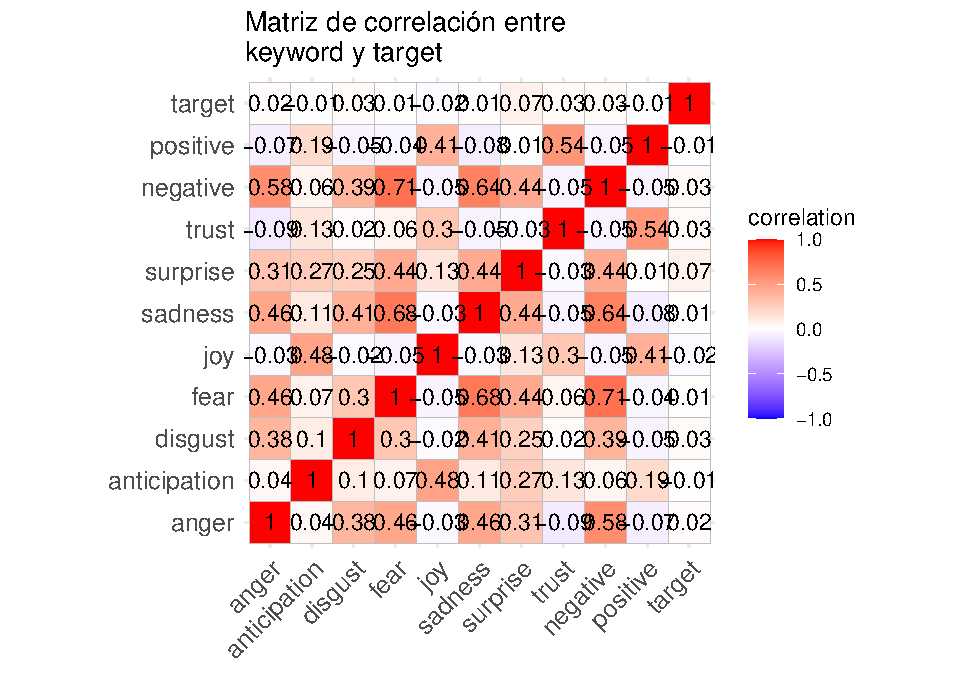
\includegraphics{exercise_files/figure-latex/unnamed-chunk-7-1} \end{center}

\begin{Shaded}
\begin{Highlighting}[]
\KeywordTok{stopCluster}\NormalTok{(cl)}
\end{Highlighting}
\end{Shaded}

Parece que, al observar la matriz de correlaciones, existe una
correlación nula entre las variables \textbf{keyword} y \textbf{target}.
Al revisarlo con mayor detalle, podemos observar que la mayoría de las
palabras clave no tienen un sentimiento positivo asociado. Las palabras
clave asociadas a un sentimiento se asocian negativamente (miedo o
tristeza), lo cual es bastante consistente con el problema, ya que
intentemos predecir el desastre.

Acorde a nuestro criterio esta variable explicativa no es buena para
hacer una predicción ya que no está realmente asociada con la variable a
predecir. Así que la excluiremos del procesamiento de texto.

\hypertarget{variable-location}{%
\subsection{\texorpdfstring{Variable
\emph{location}}{Variable location}}\label{variable-location}}

La variable explicativa \textbf{location} representa las ubicaciones
desde donde se generaron los tweets. Vemos las 10 primeras y el número
total de ubicaciones diferentes del conjunto de datos de train (3342
ubicaciones).

\begin{Shaded}
\begin{Highlighting}[]
\NormalTok{train }\OperatorTok\StringTok{ }\KeywordTok{select}\NormalTok{(location) }\OperatorTok\StringTok{ }\KeywordTok{unique}\NormalTok{() }\OperatorTok\StringTok{ }\KeywordTok{head}\NormalTok{(}\DecValTok{10}\NormalTok{)}
\end{Highlighting}
\end{Shaded}

\begin{verbatim}
##                         location
## 1                           <NA>
## 32                    Birmingham
## 33 Est. September 2012 - Bristol
## 34                        AFRICA
## 35              Philadelphia, PA
## 36                    London, UK
## 37                      Pretoria
## 38                  World Wide!!
## 40                Paranaque City
## 41                Live On Webcam
\end{verbatim}

\begin{Shaded}
\begin{Highlighting}[]
\KeywordTok{count}\NormalTok{(train }\OperatorTok\StringTok{ }\KeywordTok{select}\NormalTok{(location) }\OperatorTok\StringTok{ }\KeywordTok{unique}\NormalTok{())}
\end{Highlighting}
\end{Shaded}

\begin{verbatim}
##      n
## 1 3342
\end{verbatim}

A continuación, veremos las ubicaciones que se repiten más de 10 veces
en el conjunto de datos de train.

\begin{Shaded}
\begin{Highlighting}[]
\NormalTok{location.freq <-}\StringTok{ }\KeywordTok{table}\NormalTok{(}\KeywordTok{unlist}\NormalTok{(train }\OperatorTok\StringTok{ }\KeywordTok{select}\NormalTok{(location)))}
\NormalTok{location.freq[}\KeywordTok{which}\NormalTok{(location.freq }\OperatorTok{>}\StringTok{ }\DecValTok{10}\NormalTok{)]}
\end{Highlighting}
\end{Shaded}

\begin{verbatim}
## 
##         Australia        California   California, USA            Canada 
##                18                17                15                29 
##           Chicago       Chicago, IL             Earth        Everywhere 
##                11                18                11                15 
##           Florida             India         Indonesia           Ireland 
##                14                24                13                12 
##             Kenya            London       Los Angeles   Los Angeles, CA 
##                20                45                13                26 
##            Mumbai          New York      New York, NY           Nigeria 
##                22                71                15                28 
##               NYC     San Francisco San Francisco, CA           Seattle 
##                12                14                11                11 
##           Toronto                UK    United Kingdom     United States 
##                12                27                14                50 
##               USA  Washington, D.C.    Washington, DC         Worldwide 
##               104                13                21                19
\end{verbatim}

\begin{Shaded}
\begin{Highlighting}[]
\KeywordTok{barplot}\NormalTok{(location.freq[}\KeywordTok{which}\NormalTok{(location.freq}\OperatorTok{>}\DecValTok{10}\NormalTok{)], }\DataTypeTok{las =} \DecValTok{2}\NormalTok{,  }
        \DataTypeTok{ylab =} \StringTok{"frequency"}\NormalTok{)}
\end{Highlighting}
\end{Shaded}

\begin{center}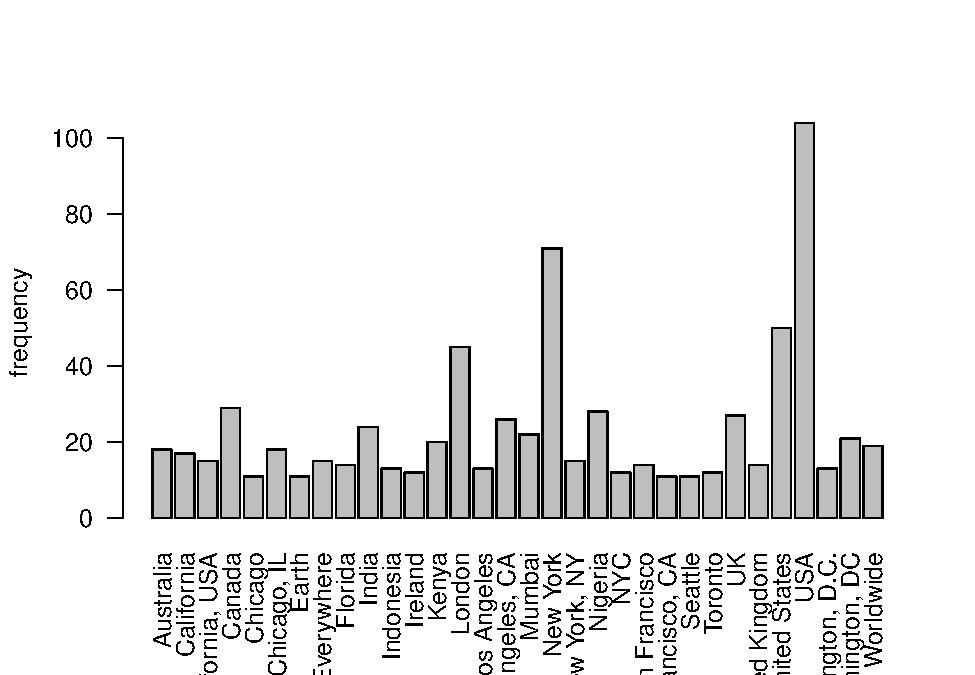
\includegraphics[width=0.7\linewidth]{exercise_files/figure-latex/unnamed-chunk-9-1} \end{center}

En el total de ubicaciones, 3342, la mayoría de ellas cuenta con menos
de 10 observaciones. Acorde a nuestro criterio esta variable explicativa
no es buena para hacer una predicción, ya que la variable tiene muy
pocas observaciones, y puede ocurrir que, durante la validación cruzada
o \emph{bootstrapping}, algunas de las particiones no contengan ninguna
observación de dicha variable, lo que puede dar lugar a errores.

\hypertarget{variable-id}{%
\subsection{\texorpdfstring{Variable
\emph{id}}{Variable id}}\label{variable-id}}

La variable \textbf{id} es solo un identificador único, así que, no la
analizaremos y procederemos a eliminarla de los conjuntos de datos de
train y test.

\begin{Shaded}
\begin{Highlighting}[]
\NormalTok{train}\OperatorTok{$}\NormalTok{id <-}\StringTok{ }\OtherTok{NULL}
\NormalTok{test}\OperatorTok{$}\NormalTok{id <-}\StringTok{ }\OtherTok{NULL}
\end{Highlighting}
\end{Shaded}

\hypertarget{conclusiuxf3n-anuxe1lisis-exploratorio}{%
\subsection{Conclusión análisis
exploratorio}\label{conclusiuxf3n-anuxe1lisis-exploratorio}}

Llegados a este punto, parece que nuestro criterio en la exploración de
los datos, el estudio de su distribución y sus posibles relaciones con
la variable a predecir nos indica que las variables explicativas
\textbf{keyword}, \textbf{location} y \textbf{id} no son buenas para
hacer una predicción, así que nos centraremos en la variable
\textbf{text} para hacer la predicción.

\hypertarget{procesamiento-de-texto}{%
\section{Procesamiento de texto}\label{procesamiento-de-texto}}

Combinamos los conjuntos de datos de train y test para ahorrar esfuerzos
en el preprocesado de datos. Para ello, usamos la función
\textbf{bind\_rows}, que nos permitirá enlazar de forma eficiente los
conjuntos de datos por fila y columna. Podremos comprobar que la
combinación se hace correctamente, sumando los elementos de train (7613)
y de test (3263), el nuevo conjunto de datos (\textbf{complete\_df})
tendrá 10876 observaciones, 3 variables explicativas (\textbf{keyword},
\textbf{location}, \textbf{text}) y la variable de clase
\textbf{target}.

\begin{Shaded}
\begin{Highlighting}[]
\NormalTok{complete_df <-}\StringTok{ }\KeywordTok{bind_rows}\NormalTok{(train, test)}
\KeywordTok{str}\NormalTok{(complete_df, }\DataTypeTok{width =} \DecValTok{85}\NormalTok{, }\DataTypeTok{strict.width =} \StringTok{"cut"}\NormalTok{)}
\end{Highlighting}
\end{Shaded}

\begin{verbatim}
## 'data.frame':    10876 obs. of  4 variables:
##  $ keyword : chr  NA NA NA NA ...
##  $ location: chr  NA NA NA NA ...
##  $ text    : chr  "Our Deeds are the Reason of this #earthquake May ALLAH Forgive "..
##  $ target  : Factor w/ 2 levels "No","Yes": 2 2 2 2 2 2 2 2 2 2 ...
\end{verbatim}

El preprocesado de datos englobará las transformaciones de los textos,
como, por ejemplo, la imputación de valores ausentes o la reducción de
dimensionalidad.

Primero, miramos cuantos valores perdidos tiene nuestro conjunto de
datos \textbf{complete\_df}. La función \textbf{colSums} sumará los
valores que la función \textbf{sapply} encuentre, en este caso, los
valores perdidos.

\begin{Shaded}
\begin{Highlighting}[]
\KeywordTok{colSums}\NormalTok{(}\KeywordTok{sapply}\NormalTok{(complete_df, is.na))}
\end{Highlighting}
\end{Shaded}

\begin{verbatim}
##  keyword location     text   target 
##       87     3638        0     3263
\end{verbatim}

Identificamos que las variables explicativas \textbf{keyword} y
\textbf{location} tienen valores perdidos. La variable explicativa
\textbf{text} no tiene valores perdidos. Sobretodo hay una gran cantidad
de tweets, para los cuales falta su ubicación. Los 3263 valores perdidos
de la variable a predecir provienen del conjunto de datos de test. Nos
ocuparemos de los valores perdidos más adelante.

\hypertarget{corpus}{%
\subsection{Corpus}\label{corpus}}

Con nuestro nuevo conjunto de datos preparado (\textbf{complete\_df}),
procedemos a crear nuestro Corpus, es decir, el conjunto de textos de la
variable \textbf{text} a analizar. En este caso, nuestro Corpus se
compone de todos los textos de los tweets y los asignaremos al objeto
\emph{myCorpus} usando las funciones \textbf{VectorSource} y
\textbf{Corpus}. La función \textbf{Corpus} creará el corpus a partir de
un vector de textos. La función \textbf{VectorSource} interpretará cada
mensaje de texto de los tweets como un elemento de ese vector de textos.

\emph{Un corpus lingüístico se define como ``un conjunto de textos de un
mismo origen'' y que tiene por función recopilar un conjunto de textos.
El uso de un corpus lingüístico nos permitirá obtener información de las
palabras utilizadas con más o menor frecuencia.}

\begin{Shaded}
\begin{Highlighting}[]
\NormalTok{myCorpus <-}\StringTok{ }\KeywordTok{Corpus}\NormalTok{(}\KeywordTok{VectorSource}\NormalTok{(complete_df}\OperatorTok{$}\NormalTok{text))}
\NormalTok{myCorpus}
\end{Highlighting}
\end{Shaded}

\begin{verbatim}
## <<SimpleCorpus>>
## Metadata:  corpus specific: 1, document level (indexed): 0
## Content:  documents: 10876
\end{verbatim}

Como podemos ver, nuestro Corpus está compuesto por 10876 textos.

\hypertarget{limpieza-del-texto}{%
\subsection{Limpieza del texto}\label{limpieza-del-texto}}

Necesitamos limpiar de los 10876 textos caracteres que son de poca
utilidad. Empezamos por aseguramos de que no queden enlaces, con un poco
de ayuda de las \emph{regular expressions}. Para ello usaremos las
funciones \textbf{gsub} y \textbf{tm\_map}. La función \textbf{gsub}
buscará y reemplazará desde la primera hasta la última de las
coincidencias de un patrón (representado por una \emph{regular
expression}). La función \textbf{tm\_map} será la encargada de aplicar
las diferentes transformaciones de los textos a nuestro corpus.

\emph{Una expresión regular (o en inglés regular expression) es una
representación, según unas reglas sintácticas de un lenguaje formal, de
una porción de texto genérico a buscar dentro de otro texto, como por
ejemplo caracteres, palabras o patrones de texto concretos.}

\begin{Shaded}
\begin{Highlighting}[]
\NormalTok{removeURL <-}\StringTok{ }\ControlFlowTok{function}\NormalTok{(x) }\KeywordTok{gsub}\NormalTok{(}\StringTok{"http[^[:space:]]*"}\NormalTok{, }\StringTok{""}\NormalTok{, x)  }
\NormalTok{myCorpus <-}\StringTok{ }\KeywordTok{tm_map}\NormalTok{(myCorpus, }\KeywordTok{content_transformer}\NormalTok{(removeURL))}
\end{Highlighting}
\end{Shaded}

Convertimos todo a minúsculas.

\begin{Shaded}
\begin{Highlighting}[]
\NormalTok{myCorpus <-}\StringTok{ }\KeywordTok{tm_map}\NormalTok{(myCorpus, }\KeywordTok{content_transformer}\NormalTok{(tolower))}
\end{Highlighting}
\end{Shaded}

Eliminamos los nombres de usuario.

\begin{Shaded}
\begin{Highlighting}[]
\NormalTok{removeUsername <-}\StringTok{ }\ControlFlowTok{function}\NormalTok{(x) }\KeywordTok{gsub}\NormalTok{(}\StringTok{"@[^[:space:]]*"}\NormalTok{, }\StringTok{""}\NormalTok{, x)  }
\NormalTok{myCorpus <-}\StringTok{ }\KeywordTok{tm_map}\NormalTok{(myCorpus, }\KeywordTok{content_transformer}\NormalTok{(removeUsername))}
\end{Highlighting}
\end{Shaded}

Nos deshacemos de la puntuación, puesto que por ejemplo ``fin'' y
``fin.'' son identificadas como palabras diferentes, lo cual no
deseamos.

\begin{Shaded}
\begin{Highlighting}[]
\NormalTok{removeNumPunct <-}\StringTok{ }\ControlFlowTok{function}\NormalTok{(x) }\KeywordTok{gsub}\NormalTok{(}\StringTok{"[^[:alpha:][:space:]]*"}\NormalTok{, }\StringTok{""}\NormalTok{, x)   }
\NormalTok{myCorpus <-}\StringTok{ }\KeywordTok{tm_map}\NormalTok{(myCorpus, }\KeywordTok{content_transformer}\NormalTok{(removeNumPunct))}
\end{Highlighting}
\end{Shaded}

Usamos \textbf{removeWords} con \textbf{stopwords(``english'')},
recordemos que los textos de los tweets están en inglés y cada idioma
tiene sus propias palabras vacías; para eliminar palabras vacías, es
decir, aquellas con poco valor para el análisis, que carecen de un
significado por si solas, tales como artículos, preposiciones,
conjunciones, pronombres, etc.

\begin{Shaded}
\begin{Highlighting}[]
\NormalTok{myStopWords <-}\StringTok{ }\KeywordTok{c}\NormalTok{((}\KeywordTok{stopwords}\NormalTok{(}\StringTok{'english'}\NormalTok{)), }
    \KeywordTok{c}\NormalTok{(}\StringTok{"really"}\NormalTok{, }\StringTok{"tweets"}\NormalTok{, }\StringTok{"saw"}\NormalTok{, }\StringTok{"just"}\NormalTok{, }\StringTok{"feel"}\NormalTok{, }\StringTok{"may"}\NormalTok{, }\StringTok{"us"}\NormalTok{, }\StringTok{"rt"}\NormalTok{, }\StringTok{"every"}\NormalTok{, }\StringTok{"one"}\NormalTok{,}
     \StringTok{"amp"}\NormalTok{, }\StringTok{"like"}\NormalTok{, }\StringTok{"will"}\NormalTok{, }\StringTok{"got"}\NormalTok{, }\StringTok{"new"}\NormalTok{, }\StringTok{"can"}\NormalTok{, }\StringTok{"still"}\NormalTok{, }\StringTok{"back"}\NormalTok{, }\StringTok{"top"}\NormalTok{, }\StringTok{"much"}\NormalTok{,}
     \StringTok{"near"}\NormalTok{, }\StringTok{"im"}\NormalTok{, }\StringTok{"see"}\NormalTok{, }\StringTok{"via"}\NormalTok{, }\StringTok{"get"}\NormalTok{, }\StringTok{"now"}\NormalTok{, }\StringTok{"come"}\NormalTok{, }\StringTok{"oil"}\NormalTok{, }\StringTok{"let"}\NormalTok{, }\StringTok{"god"}\NormalTok{, }\StringTok{"want"}\NormalTok{,}
     \StringTok{"pm"}\NormalTok{, }\StringTok{"last"}\NormalTok{, }\StringTok{"hope"}\NormalTok{, }\StringTok{"since"}\NormalTok{, }\StringTok{"everyone"}\NormalTok{, }\StringTok{"food"}\NormalTok{, }\StringTok{"content"}\NormalTok{, }\StringTok{"always"}\NormalTok{, }\StringTok{"th"}\NormalTok{,}
     \StringTok{"full"}\NormalTok{, }\StringTok{"found"}\NormalTok{, }\StringTok{"dont"}\NormalTok{, }\StringTok{"look"}\NormalTok{, }\StringTok{"cant"}\NormalTok{, }\StringTok{"mh"}\NormalTok{, }\StringTok{"lol"}\NormalTok{, }\StringTok{"set"}\NormalTok{, }\StringTok{"old"}\NormalTok{, }\StringTok{"service"}\NormalTok{,}
     \StringTok{"city"}\NormalTok{, }\StringTok{"home"}\NormalTok{, }\StringTok{"live"}\NormalTok{, }\StringTok{"night"}\NormalTok{, }\StringTok{"news"}\NormalTok{, }\StringTok{"say"}\NormalTok{, }\StringTok{"video"}\NormalTok{, }\StringTok{"people"}\NormalTok{, }\StringTok{"ill"}\NormalTok{, }
     \StringTok{"way"}\NormalTok{,  }\StringTok{"please"}\NormalTok{, }\StringTok{"years"}\NormalTok{, }\StringTok{"take"}\NormalTok{, }\StringTok{"homes"}\NormalTok{, }\StringTok{"read"}\NormalTok{, }\StringTok{"man"}\NormalTok{, }\StringTok{"next"}\NormalTok{, }\StringTok{"cross"}\NormalTok{, }
     \StringTok{"boy"}\NormalTok{, }\StringTok{"bad"}\NormalTok{, }\StringTok{"ass"}\NormalTok{))}

\KeywordTok{head}\NormalTok{(myStopWords, }\DecValTok{30}\NormalTok{)}
\end{Highlighting}
\end{Shaded}

\begin{verbatim}
##  [1] "i"          "me"         "my"         "myself"     "we"        
##  [6] "our"        "ours"       "ourselves"  "you"        "your"      
## [11] "yours"      "yourself"   "yourselves" "he"         "him"       
## [16] "his"        "himself"    "she"        "her"        "hers"      
## [21] "herself"    "it"         "its"        "itself"     "they"      
## [26] "them"       "their"      "theirs"     "themselves" "what"
\end{verbatim}

\begin{Shaded}
\begin{Highlighting}[]
\NormalTok{myCorpus <-}\StringTok{ }\KeywordTok{tm_map}\NormalTok{(myCorpus, removeWords, myStopWords) }
\end{Highlighting}
\end{Shaded}

Además, podemos ver que se han añadido (aleatoriamente) más palabras
vacías (``really'', ``tweets'', ``saw'', etc.). Estas palabras vacías
son de las más usadas en los mensajes de texto de los tweets (ver
\url{https://techland.time.com/2009/06/08/the-500-most-frequently-used-words-on-twitter/}).

En este caso, removemos las palabras de una sola letra.

\begin{Shaded}
\begin{Highlighting}[]
\NormalTok{removeSingle <-}\StringTok{ }\ControlFlowTok{function}\NormalTok{(x) }\KeywordTok{gsub}\NormalTok{(}\StringTok{" . "}\NormalTok{, }\StringTok{" "}\NormalTok{, x)   }
\NormalTok{myCorpus <-}\StringTok{ }\KeywordTok{tm_map}\NormalTok{(myCorpus, }\KeywordTok{content_transformer}\NormalTok{(removeSingle))}
\end{Highlighting}
\end{Shaded}

Por último eliminamos los espacios vacíos excesivos, muchos de ellos
introducidos por las transformaciones anteriores.

\begin{Shaded}
\begin{Highlighting}[]
\NormalTok{myCorpus <-}\StringTok{ }\KeywordTok{tm_map}\NormalTok{(myCorpus, stripWhitespace)}
\end{Highlighting}
\end{Shaded}

\hypertarget{creaciuxf3n-de-un-modelo-predictivo}{%
\section{Creación de un modelo
predictivo}\label{creaciuxf3n-de-un-modelo-predictivo}}

\hypertarget{preprocesado-de-los-datos}{%
\subsection{Preprocesado de los datos}\label{preprocesado-de-los-datos}}

Para la creación de un modelo predictivo, necesitamos construir una
\textbf{Term Document Matrix} del conjunto de textos de la variable
\textbf{text}, donde cada fila representará un texto y cada palabra
única estará representada per una columna.

\emph{Una Term Document Matrix es una matriz matemática que describe la
frecuencia con la que se repiten una serie de palabras en una colección
de documentos.}

Comenzaremos mapeando nuestro Corpus indicando que es una \textbf{Term
Document Matrix}, de esta manera podremos realizar el preprocesado de
datos. Sabemos que el preprocesado de datos engloba aquellas
transformaciones de los datos con la finalidad de mejorar los resultados
de la clasificación supervisada. Todo preprocesado de datos debe
aprenderse de las observaciones de train y luego aplicarse al conjunto
de train y de test. Esto es muy importante para no violar la condición
de que ninguna información procedente de las observaciones de test
influya en el ajuste del modelo.

Utilizaremos la función \textbf{TermDocumentMatrix} en nuestro Corpus y
asignaremos el resultado al objeto \emph{complete.tdm}. Con el parámetro
\textbf{control} indicaremos que evaluaremos todos los textos de la
matriz, con las características escogidas se evaluarán todas las
palabras de los textos. Por defecto la función
\textbf{TermDocumentMatrix} usa \emph{tf-id}, que mide la importancia
relativa de cada palabra en el conjunto de textos.

\begin{Shaded}
\begin{Highlighting}[]
\NormalTok{complete.tdm <-}\StringTok{ }\KeywordTok{TermDocumentMatrix}\NormalTok{(myCorpus, }\DataTypeTok{control=}\KeywordTok{list}\NormalTok{(}\DataTypeTok{wordLengths=} \KeywordTok{c}\NormalTok{(}\DecValTok{4}\NormalTok{, }\OtherTok{Inf}\NormalTok{)))}
\NormalTok{complete.tdm}
\end{Highlighting}
\end{Shaded}

\begin{verbatim}
## <<TermDocumentMatrix (terms: 16880, documents: 10876)>>
## Non-/sparse entries: 76219/183510661
## Sparsity           : 100%
## Maximal term length: 49
## Weighting          : term frequency (tf)
\end{verbatim}

Podemos observar que tenemos 16880 \emph{terms}, esto quiere decir que
tenemos 16880 palabras diferentes en nuestro Corpus. Lo cual es una
cantidad considerable de vocabulario, pero no esperaríamos otra cosa de
una red social como \href{https://twitter.com}{Twitter}. La palabra más
larga contiene 49 caracteres.

Usaremos la función \textbf{removeSparseItems} para depurar nuestra
\textbf{Term Document Matrix} de aquellas palabras que aparecen con muy
poca frecuencia, es decir, son dispersas. Porqué 16880 palabras son
demasiadas palabras y es posible que no podamos entrenar nuestro modelo
debido a restricciones computacionales.

Esta función requiere que especifiquemos el argumento \textbf{sparse},
que puede asumir valores de 0 a 1. Este valor representa la dispersión
de las palabras que queremos conservar. Si lo fijamos muy alto (cerca de
1, pero no 1), conservaremos muchas palabras, casi todas, pues estamos
indicando que queremos conservar palabras, aunque sean muy dispersas.
Naturalmente, ocurre lo opuesto si fijamos este valor muy bajo (cerca de
0, pero no 0), pudiendo incluso quedarnos sin ninguna palabra, si las
palabras en nuestros textos son dispersas en general.

En este caso, se decide fijarlo en \emph{.9975}, conservando las
palabras que aparecen en al menos el 0.25\% de las observaciones.

\begin{Shaded}
\begin{Highlighting}[]
\NormalTok{complete.tdm <-}\StringTok{ }\KeywordTok{removeSparseTerms}\NormalTok{(complete.tdm, }\DataTypeTok{sparse =} \FloatTok{.9975}\NormalTok{)}
\NormalTok{complete.tdm}
\end{Highlighting}
\end{Shaded}

\begin{verbatim}
## <<TermDocumentMatrix (terms: 582, documents: 10876)>>
## Non-/sparse entries: 31214/6298618
## Sparsity           : 100%
## Maximal term length: 17
## Weighting          : term frequency (tf)
\end{verbatim}

De 16880 palabras que teníamos, nos hemos quedado con 582, lo cual
reduce en gran medida la dificultad y complejidad del problema de
\emph{alta dimensionalidad}, lo cual es deseable. La palabra más larga
contiene 17 caracteres.

\hypertarget{feature-extraction-mediante-singular-value-decomposition-svd}{%
\subsubsection{Feature Extraction mediante Singular Value Decomposition
(SVD)}\label{feature-extraction-mediante-singular-value-decomposition-svd}}

La descomposición de los datos originales en un nuevo conjunto, sin
necesidad de pérdida de información relevante y sacando a la luz la
información latente, es un proceso de vital importancia para implementar
la parte más computacionalmente intensa del ejercicio. Buscando una
intuitiva separabilidad de las clases de los datos aplicaremos la
técnica de \emph{Descomposición en Valores Singulares (SVD)}.

\emph{La Descomposición de Valores Singulares (en inglés Singular Value
Decomposition ({[}SVD{]}
(\url{https://en.wikipedia.org/wiki/Singular-value_decomposition})) es
una técnica de reducción de la dimensionalidad, en minería de textos,
que puede utilizarse para descubrir las dimensiones latentes (o
componentes) que determinan similitudes semánticas entre las palabras
(es decir, unidades léxicas) o entre los textos (es decir, unidades de
contexto).}

Para aplicar la técnica de \emph{Descomposición en Valores Singulares
(SVD)}, primero transformamos nuestra \textbf{Term Document Matrix} a un
objeto de tipo \textbf{matrix} para así poder comprobar si nuestros
datos aún contienen valores perdidos con la función \textbf{which}.

\begin{verbatim}
## integer(0)
\end{verbatim}

Los datos no contienen valores perdidos, podemos proceder con la
\emph{Descomposición de Valores Singulares (SVD)}. Para ello utilizamos
la función \textbf{irlba}, que se encargará de la descomposición de
nuestra \textbf{Term Document Matrix} y extraerá sus 150 vectores
singulares más importantes, después de un máximo de 600 iteraciones, y
que guardaremos en el objeto \textbf{complete\_irlba}.

\begin{Shaded}
\begin{Highlighting}[]
\NormalTok{cl <-}\StringTok{ }\KeywordTok{makePSOCKcluster}\NormalTok{(}\DecValTok{4}\NormalTok{, }\DataTypeTok{setup_strategy=}\StringTok{"sequential"}\NormalTok{)}
\KeywordTok{registerDoParallel}\NormalTok{(cl)}

\NormalTok{complete_irlba <-}\StringTok{ }\KeywordTok{irlba}\NormalTok{(}\KeywordTok{t}\NormalTok{(complete.term.matrix), }\DataTypeTok{nv =} \DecValTok{150}\NormalTok{, }\DataTypeTok{maxit =} \DecValTok{600}\NormalTok{)}
\NormalTok{complete_irlba}\OperatorTok{$}\NormalTok{v[}\DecValTok{1}\OperatorTok{:}\DecValTok{10}\NormalTok{, }\DecValTok{1}\OperatorTok{:}\DecValTok{5}\NormalTok{]}
\end{Highlighting}
\end{Shaded}

\begin{verbatim}
##                [,1]          [,2]          [,3]          [,4]          [,5]
##  [1,] -0.0003162281 -2.109638e-04  3.318231e-04  2.035137e-05 -0.0008660149
##  [2,] -0.0431207327  1.408993e-02 -5.124787e-03 -3.922969e-03  0.0021251369
##  [3,] -0.0020297768  2.205792e-04  5.231801e-05 -1.014223e-04 -0.0008899277
##  [4,] -0.0054444920  1.259299e-04  3.441743e-03 -1.669137e-04 -0.0094345444
##  [5,] -0.0021975777  8.533917e-05 -7.910354e-05  7.809264e-05 -0.0017043646
##  [6,] -0.0449020384  1.303972e-02 -1.677561e-03 -3.883599e-03  0.0005116573
##  [7,] -0.0060579030 -8.521515e-03  3.239198e-02 -6.490016e-04  0.0023784289
##  [8,] -0.0387247287  1.297783e-02 -5.140001e-03 -3.764856e-03  0.0112714576
##  [9,] -0.0079142623 -5.649745e-04  6.691751e-04  4.606357e-04 -0.0135358450
## [10,] -0.0014005942 -2.762898e-04  3.440679e-04  4.573951e-05 -0.0016280077
\end{verbatim}

\begin{Shaded}
\begin{Highlighting}[]
\KeywordTok{stopCluster}\NormalTok{(cl)}
\end{Highlighting}
\end{Shaded}

Lo que vemos arriba es una pequeña parte del modelo de espacio vectorial
de los 150 vectores singulares más importantes, que usaremos como
características para la clasificación supervisada.

\hypertarget{divisiuxf3n-de-los-datos-en-train-y-test}{%
\subsection{División de los datos en train y
test}\label{divisiuxf3n-de-los-datos-en-train-y-test}}

Evaluar la capacidad predictiva de un modelo consiste en comprobar cómo
de próximas son sus predicciones a los verdaderos valores de la variable
a predecir. Para poder cuantificar de forma correcta este error, se
necesita disponer de un conjunto de observaciones, de las que se conozca
la variable a predecir, pero que el modelo no haya ``visto'', es decir,
que no hayan participado en su ajuste. Con esta finalidad, se dividen
los datos disponibles en un conjunto de train y un conjunto de test.

Con el conjunto de datos, del que se conoce la variable a predecir
(\textbf{complete\_df}) y las características que hemos creado en la
sección anterior (\textbf{complete\_irlba}) creamos un nuevo conjunto de
datos que a continuación dividiremos en un conjunto de datos de train
(\textbf{train.df}) y de test (\textbf{test.df}), con el mismo tamaño de
la partición inicial proporcionada por la competición de Kaggle (7613
instancias para el conjunto de datos de train y 3263 instancias para el
conjunto de datos de test).

\begin{Shaded}
\begin{Highlighting}[]
\NormalTok{complete.svd <-}\StringTok{ }\KeywordTok{data.frame}\NormalTok{(}\DataTypeTok{target=}\NormalTok{complete_df}\OperatorTok{$}\NormalTok{target, complete_irlba}\OperatorTok{$}\NormalTok{v)}
\NormalTok{train.df <-}\StringTok{ }\NormalTok{complete.svd[}\DecValTok{1}\OperatorTok{:}\DecValTok{7613}\NormalTok{, ]}
\NormalTok{test.df <-}\StringTok{ }\NormalTok{complete.svd[}\DecValTok{7614}\OperatorTok{:}\DecValTok{10876}\NormalTok{, }\DecValTok{-1}\NormalTok{]}
\KeywordTok{dim}\NormalTok{(train.df)}
\end{Highlighting}
\end{Shaded}

\begin{verbatim}
## [1] 7613  151
\end{verbatim}

\begin{Shaded}
\begin{Highlighting}[]
\KeywordTok{dim}\NormalTok{(test.df)}
\end{Highlighting}
\end{Shaded}

\begin{verbatim}
## [1] 3263  150
\end{verbatim}

Un paso importante es verificar que la distribución de la variable a
predecir del conjunto datos de train no ha cambiado respecto a la
partición inicial (\textbf{complete\_df}).

\begin{Shaded}
\begin{Highlighting}[]
\KeywordTok{prop.table}\NormalTok{(}\KeywordTok{table}\NormalTok{(complete_df}\OperatorTok{$}\NormalTok{target))}
\end{Highlighting}
\end{Shaded}

\begin{verbatim}
## 
##        No       Yes 
## 0.5703402 0.4296598
\end{verbatim}

\begin{Shaded}
\begin{Highlighting}[]
\KeywordTok{prop.table}\NormalTok{(}\KeywordTok{table}\NormalTok{(train.df}\OperatorTok{$}\NormalTok{target))}
\end{Highlighting}
\end{Shaded}

\begin{verbatim}
## 
##        No       Yes 
## 0.5703402 0.4296598
\end{verbatim}

\hypertarget{selecciuxf3n-de-variables}{%
\subsection{Selección de variables}\label{selecciuxf3n-de-variables}}

Cuando se entrena un modelo, es importante incluir como variables para
la predicción únicamente aquellas variables que están realmente
relacionadas con la variable a predecir, ya que son estas las que
contienen información útil para el modelo. Incluir un exceso de
variables suele conllevar una reducción de la capacidad de predicción
del modelo. La selección de variables para la predicción puede suponer
la diferencia entre un modelo normal y uno muy bueno, por lo tanto,
conviene conocer las herramientas internas de *caret** para la selección
de variables.

Muchos modelos a los que se puede acceder mediante la función
\textbf{train} de \textbf{caret} producen ecuaciones de predicción que
no necesariamente utilizan todas las variables. Estos modelos tienen una
selección de variables incorporada. El uso de estos modelos con
selección de variables incorporada será más eficiente que otras
estrategias, de wrapper y filtrado.

Para este ejercicio, escogemos algoritmos de clasificación supervisada
de \textbf{caret} que tienen una selección de variables incorporada (ver
\url{http://topepo.github.io/caret/feature-selection-overview.html})..

\hypertarget{entrenamiento-de-modelos}{%
\subsection{Entrenamiento de modelos}\label{entrenamiento-de-modelos}}

En esta sección se entrenan diferentes modelos de \emph{clasificación
supervisada} con el objetivo de compararlos e identificar el que mejor
resultado obtiene prediciendo. Todos estos modelos incorporados en el
paquete \textbf{caret} se entrenan con la función \textbf{train}. Entre
los argumentos de esta función destacan:

\begin{itemize}
\item
  \textbf{method}. El nombre del algoritmo que se desea emplear
  (\href{http://topepo.github.io/caret/available-models.html}{modelos}.
\item
  \textbf{metric}. La métrica empleada para evaluar la capacidad
  predictiva del modelo. Aunque la competición de Kaggle en la que se
  basa nuestro ejercicio usa \textbf{F1 score} como métrica de
  evaluación, para cuantificar como de bueno son los modelos
  utilizaremos la métrica de evaluación \emph{Accuracy}. Porqué la
  distribución de la clase no presenta un problema notable de
  desbalanceo de clases y cuando la distribución de la variable clase
  está bastante equilibrada es una buena medida de evaluación.
\end{itemize}

\emph{Accuracy representa el porcentaje total de elementos clasificados
correctamente. Es la medida más directa de la calidad de los
clasificadores. Es un valor entre 0 y 1. Cuanto más alto, mejor.}

\begin{itemize}
\tightlist
\item
  \textbf{trControl}. Especificaciones adicionales sobre la forma de
  llevar a cabo el entrenamiento del modelo.
\end{itemize}

La función \textbf{train} de \textbf{caret} siempre estima un porcentaje
de bien clasificados sobre el conjunto de datos de train. La función
\textbf{trainControl}, que se pasa al argumento \textbf{trControl} de la
función \textbf{train}, controla la estimación del error: en este caso
realizaremos una \emph{K-Fold Cross-Validation} usando la función
\textbf{createMultiFolds}, de 5 hojas (\emph{k}) y repitiéndola 3 veces
(\emph{times}). Una validación cruzada con 5 hojas y 3 repeticiones,
implica ajustar y evaluar el modelo 5 * 3 = 15 veces, más un último
ajuste con todos los datos de entrenamiento para crear el modelo final.

\emph{La Cross-validation se emplea para estimar el test error rate de
un modelo y así evaluar su capacidad predictiva. Específicamente, el
método K-Fold Cross-Validation es un proceso iterativo. Consiste en
dividir los datos de forma aleatoria en k grupos de aproximadamente el
mismo tamaño. k-1 grupos se emplean para entrenar el modelo y uno de los
grupos se emplea como test, este proceso se repite k veces utilizando un
grupo distinto como test en cada iteración. El proceso genera k
estimaciones del test error cuyo promedio se emplea como estimación
final.}

Las semillas son necesarias si se quiere asegurar la reproducibilidad de
los resultados, ya que una validación cruzada implica una selección
aleatoria.

\begin{Shaded}
\begin{Highlighting}[]
\KeywordTok{set.seed}\NormalTok{(}\DecValTok{123}\NormalTok{)}
\NormalTok{cv.folds <-}\StringTok{ }\KeywordTok{createMultiFolds}\NormalTok{(train.df}\OperatorTok{$}\NormalTok{target, }\DataTypeTok{k=}\DecValTok{5}\NormalTok{, }\DataTypeTok{times=}\DecValTok{3}\NormalTok{)}
\NormalTok{cv.cntrl <-}\StringTok{ }\KeywordTok{trainControl}\NormalTok{(}\DataTypeTok{method=}\StringTok{"repeatecv"}\NormalTok{, }\DataTypeTok{number=}\DecValTok{5}\NormalTok{,}
                         \DataTypeTok{index=}\NormalTok{cv.folds, }\DataTypeTok{allowParallel=}\OtherTok{TRUE}\NormalTok{, }
                         \DataTypeTok{returnResamp=}\StringTok{"final"}\NormalTok{,}
                         \DataTypeTok{verboseIter=}\OtherTok{FALSE}\NormalTok{)}
\end{Highlighting}
\end{Shaded}

El argumento \textbf{method} de la función \textbf{trainControl} hace
posible utilizar distintos tipos de validación. En este caso es
\emph{repeatecv} (para entrenamiento repetido/división de test). Además
de fijar el tipo de validación, la función \textbf{trainControl} permite
fijar multitud de argumentos. A continuación, describimos los que se han
fijado:

\begin{itemize}
\tightlist
\item
  \textbf{number}. El número de hojas (\emph{5}).
\item
  \textbf{index}. Lista con los elementos para cada iteración
  (\textbf{cv.folds}). Cada elemento de la lista es un vector de números
  enteros correspondientes a las filas utilizadas para el entrenamiento
  en esa iteración.
\end{itemize}

\begin{Shaded}
\begin{Highlighting}[]
\KeywordTok{str}\NormalTok{(cv.folds)}
\end{Highlighting}
\end{Shaded}

\begin{verbatim}
## List of 15
##  $ Fold1.Rep1: int [1:6090] 1 2 3 4 5 6 7 8 9 11 ...
##  $ Fold2.Rep1: int [1:6090] 1 2 3 4 5 7 8 9 10 11 ...
##  $ Fold3.Rep1: int [1:6090] 1 2 3 5 6 7 8 9 10 11 ...
##  $ Fold4.Rep1: int [1:6091] 2 3 4 6 10 12 13 14 15 16 ...
##  $ Fold5.Rep1: int [1:6091] 1 4 5 6 7 8 9 10 11 12 ...
##  $ Fold1.Rep2: int [1:6090] 1 4 5 6 8 9 10 11 12 13 ...
##  $ Fold2.Rep2: int [1:6090] 2 3 4 5 6 7 8 9 11 12 ...
##  $ Fold3.Rep2: int [1:6090] 1 2 3 5 6 7 10 11 12 14 ...
##  $ Fold4.Rep2: int [1:6091] 1 2 3 4 5 6 7 8 9 10 ...
##  $ Fold5.Rep2: int [1:6091] 1 2 3 4 7 8 9 10 11 12 ...
##  $ Fold1.Rep3: int [1:6091] 1 2 3 6 7 8 9 10 11 12 ...
##  $ Fold2.Rep3: int [1:6090] 1 2 4 5 6 7 9 10 11 13 ...
##  $ Fold3.Rep3: int [1:6090] 1 3 4 5 8 9 10 11 12 13 ...
##  $ Fold4.Rep3: int [1:6090] 2 3 4 5 6 7 8 12 13 14 ...
##  $ Fold5.Rep3: int [1:6091] 1 2 3 4 5 6 7 8 9 10 ...
\end{verbatim}

\begin{itemize}
\tightlist
\item
  \textbf{allowParallel}. Habilita la computación paralela
  (\emph{TRUE}). \textbf{caret} permite paralelizar el proceso para que
  sea más rápido.
\item
  \textbf{returnResamp}. Indica la cantidad de métricas de evaluación
  que se deben guardar. Solo los valores finales (\emph{``final''}).
\item
  \textbf{verboseIter}. Para imprimir o no el registro de entrenamiento.
  No se imprime (\emph{FALSE}).
\end{itemize}

Muchos modelos contienen parámetros que no pueden aprenderse a partir de
los datos de entrenamiento y, por lo tanto, deben de ser establecidos
por el analista. A estos se les conoce como \emph{hiperparámetros},
argumento \textbf{tunning} de \textbf{caret}. Con la función
\textbf{expand.grid} definiremos los valores de los argumentos a tunear.

Los resultados de un modelo pueden depender en gran medida del valor que
tomen sus \emph{hiperparámetros}, sin embargo, no se puede conocer de
antemano cuáles son los adecuados. La forma más común de encontrar los
valores óptimos es probando diferentes posibilidades. Para ello se
utiliza el argumento de \textbf{caret}: \textbf{tuneGrid} en la función
\textbf{train}. Si no se tiene ninguna idea de qué valores de
\emph{hiperparámetros} pueden ser los adecuados, lo mejor es utilizar la
aleatoriedad. \textbf{caret} también incorpora esta opción mediante el
argumento \textbf{tuneLength}.

En la siguiente sección realizaremos pruebas tanto con \textbf{tuneGrid}
y \textbf{tuneLength}. Más con \textbf{tuneGrid}, ya que, de esta forma,
se evita que se generen automáticamente valores que no tienen sentido o
que disparan el tiempo de computación necesario. Además, con
\emph{target \textasciitilde{}.} denotamos la variable que se quiere
predecir e indicando que el resto de las variables del conjunto de datos
de \textbf{train} son predictoras.

\hypertarget{modelos}{%
\subsection{Modelos}\label{modelos}}

Es a lo largo del proceso posterior donde más destacarán las
funcionalidades ofrecidas por \textbf{caret}, permitiendo emplear la
misma sintaxis para ajustar, optimizar, evaluar y predecir un amplio
abanico de modelos variando únicamente el nombre del algoritmo. Aunque
\textbf{caret} permite todo esto con apenas unas pocas líneas de código
son muchos los argumentos que pueden ser adaptados, cada uno con
múltiples posibilidades. Con el objetivo de exponer mejor cada una de
las opciones, en lugar de crear directamente un modelo final, se
muestran ejemplos de menor a mayor complejidad de la lista mostrada
anteriormente:
\url{http://topepo.github.io/caret/available-models.html}.

\hypertarget{regresiuxf3n-loguxedstica}{%
\subsubsection{Regresión Logística}\label{regresiuxf3n-loguxedstica}}

Información detallada sobre regresión logística en
\href{https://www.cienciadedatos.net/documentos/27_regresion_logistica_simple_y_multiple}{Regresión
logística simple y múltiple}.

\textbf{caret} emplea el método \textbf{glmnet}. Este algoritmo no tiene
ningún \emph{hiperparámetro}, por lo tanto, usamos por ejemplo
\textbf{tuneLength} igual a 15.

\begin{Shaded}
\begin{Highlighting}[]
\NormalTok{cl <-}\StringTok{ }\KeywordTok{makePSOCKcluster}\NormalTok{(}\DecValTok{6}\NormalTok{, }\DataTypeTok{setup_strategy=}\StringTok{"sequential"}\NormalTok{)}
\KeywordTok{registerDoParallel}\NormalTok{(cl)}
\end{Highlighting}
\end{Shaded}

\begin{Shaded}
\begin{Highlighting}[]
\KeywordTok{set.seed}\NormalTok{(}\DecValTok{123}\NormalTok{)}
\NormalTok{model_glmnet <-}\StringTok{ }\KeywordTok{train}\NormalTok{(target }\OperatorTok{~}\StringTok{ }\NormalTok{., }\DataTypeTok{data=}\NormalTok{train.df,}
                      \DataTypeTok{method=}\StringTok{"glmnet"}\NormalTok{,}
                      \DataTypeTok{metric=}\StringTok{"Accuracy"}\NormalTok{,}
                      \DataTypeTok{trControl=}\NormalTok{cv.cntrl,}
                      \DataTypeTok{tuneLenght=}\DecValTok{15}\NormalTok{)}
\NormalTok{model_glmnet}
\end{Highlighting}
\end{Shaded}

\begin{Shaded}
\begin{Highlighting}[]
\KeywordTok{stopCluster}\NormalTok{(cl)}
\end{Highlighting}
\end{Shaded}

El \emph{Accuracy} promedio estimado mediante validación cruzada
repetida es de 0.7650943, el modelo predice correctamente un 76.5\% de
las veces.

\hypertarget{random-forest}{%
\subsubsection{Random Forest}\label{random-forest}}

Información detallada sobre Random Forest en
\href{https://www.cienciadedatos.net/documentos/33_arboles_de_prediccion_bagging_random_forest_boosting}{Árboles
de predicción: bagging, random forest, boosting y C5.0}.

\textbf{caret} emplea el método **rf\emph{. Este algoritmo tiene un
}hiperparámetro*:

\begin{itemize}
\tightlist
\item
  \textbf{mtry}. Número de valores seleccionados aleatoriamente en cada
  árbol. En este caso hemos escogido: 3, 4, 5 y 7.
\end{itemize}

\begin{Shaded}
\begin{Highlighting}[]
\NormalTok{cl <-}\StringTok{ }\KeywordTok{makePSOCKcluster}\NormalTok{(}\DecValTok{6}\NormalTok{, }\DataTypeTok{setup_strategy=}\StringTok{"sequential"}\NormalTok{)}
\KeywordTok{registerDoParallel}\NormalTok{(cl)}
\end{Highlighting}
\end{Shaded}

\begin{Shaded}
\begin{Highlighting}[]
\KeywordTok{set.seed}\NormalTok{(}\DecValTok{123}\NormalTok{)}
\NormalTok{cv.grid <-}\StringTok{ }\KeywordTok{expand.grid}\NormalTok{(}\DataTypeTok{mtry=}\KeywordTok{c}\NormalTok{(}\DecValTok{3}\NormalTok{, }\DecValTok{4}\NormalTok{, }\DecValTok{5}\NormalTok{, }\DecValTok{7}\NormalTok{))}
\NormalTok{model_rf <-}\StringTok{ }\KeywordTok{train}\NormalTok{(target }\OperatorTok{~}\StringTok{ }\NormalTok{., }\DataTypeTok{data=}\NormalTok{train.df,}
                      \DataTypeTok{method=}\StringTok{"rf"}\NormalTok{,}
                      \DataTypeTok{metric=}\StringTok{"Accuracy"}\NormalTok{,}
                      \DataTypeTok{trControl=}\NormalTok{cv.cntrl,}
                      \DataTypeTok{tuneGrid=}\NormalTok{cv.grid)}
\NormalTok{model_rf}
\end{Highlighting}
\end{Shaded}

\begin{Shaded}
\begin{Highlighting}[]
\KeywordTok{stopCluster}\NormalTok{(cl)}
\end{Highlighting}
\end{Shaded}

Empleando un modelo Random Forest con mtry = 7 se consigue un
\emph{Accuracy} promedio de validación igual a 0.7618528, el modelo
predice correctamente un 76.2\% de las veces.

\hypertarget{gradient-boosting}{%
\subsubsection{Gradient Boosting}\label{gradient-boosting}}

Información detallada sobre boosting
\href{https://www.cienciadedatos.net/documentos/33_arboles_de_prediccion_bagging_random_forest_boosting}{Árboles
de predicción: bagging, random forest, boosting y C5.0}.

El método \textbf{gbm} de \textbf{caret} emplea el paquete gbm. Este
algoritmo tiene 4 \emph{hiperparámetros}:

\begin{itemize}
\item
  \textbf{n.trees}. Número de iteraciones del algoritmo de boosting.
  Cuanto mayor es este valor, más se reduce el error de entrenamiento.
\item
  \textbf{interaction.depth}. El número total de divisiones que tiene el
  árbol. Emplear árboles con ente 1 y 6 nodos suele dar buenos
  resultados.
\item
  \textbf{shrinkage}. Controla la complejidad que tiene el modelo. Es
  preferible mejorar un modelo mediante muchos pasos pequeños que
  mediante unos pocos grandes. Por esta razón, se emplea un valor de
  \textbf{shrinkage} tan pequeño como sea posible, teniendo en cuenta
  que, cuanto menor sea, mayor el número de iteraciones necesarias. Por
  defecto es de 0.001.
\item
  \textbf{n.minobsinnode}. Número mínimo de observaciones que debe tener
  cada nodo del árbol para poder ser dividido. Al igual que
  \textbf{interaction.depth}, permite controlar la complejidad que tiene
  el modelo.
\end{itemize}

Además de los hiperparámetros que permite controlar \textbf{caret},
tiene otros dos más que hay que tener en cuenta:

\begin{itemize}
\item
  \textbf{distribution}. Determina la función de coste (\emph{loss
  function}). Algunas de las más utilizadas son: \emph{gaussian}
  (squared loss) para regresión, \emph{bernoulli} para clasificaciones
  binarias, multinomial para clasificaciones con más de dos clases y
  \emph{adaboost} para clasificaciones binarias y que emplea la función
  exponencial del algoritmo original
  \href{https://en.wikipedia.org/wiki/AdaBoost}{AdaBoost}.
\item
  \textbf{bag.fraction} (subsampling fraction): fracción de
  observaciones del conjunto de train seleccionadas de forma aleatoria.
  Si su valor es de 1, se emplea el algoritmo de \emph{Gradient
  Boosting}, si es menor que 1, se emplea \emph{Stochastic Gradient
  Boosting}. Por defecto su valor es de 0.5.
\end{itemize}

En este caso solo añadimos el argumento \textbf{distribution} y como el
ejercicio se basa en un problema de clasificación binaria usamos
\emph{adaboost}.

\begin{Shaded}
\begin{Highlighting}[]
\KeywordTok{library}\NormalTok{(gbm)}
\end{Highlighting}
\end{Shaded}

\begin{verbatim}
## Loaded gbm 2.1.8
\end{verbatim}

\begin{Shaded}
\begin{Highlighting}[]
\NormalTok{cl <-}\StringTok{ }\KeywordTok{makePSOCKcluster}\NormalTok{(}\DecValTok{6}\NormalTok{, }\DataTypeTok{setup_strategy=}\StringTok{"sequential"}\NormalTok{)}
\KeywordTok{registerDoParallel}\NormalTok{(cl)}
\end{Highlighting}
\end{Shaded}

\begin{Shaded}
\begin{Highlighting}[]
\KeywordTok{set.seed}\NormalTok{(}\DecValTok{123}\NormalTok{)}
\NormalTok{cv.grid <-}\StringTok{ }\KeywordTok{expand.grid}\NormalTok{(}\DataTypeTok{interaction.depth=}\KeywordTok{c}\NormalTok{(}\DecValTok{1}\NormalTok{, }\DecValTok{2}\NormalTok{),}
                       \DataTypeTok{n.trees=}\DecValTok{100}\NormalTok{,}
                       \DataTypeTok{shrinkage=}\KeywordTok{c}\NormalTok{(}\FloatTok{0.001}\NormalTok{, }\FloatTok{0.01}\NormalTok{, }\FloatTok{0.1}\NormalTok{),}
                       \DataTypeTok{n.minobsinnode=}\KeywordTok{c}\NormalTok{(}\DecValTok{2}\NormalTok{, }\DecValTok{5}\NormalTok{, }\DecValTok{15}\NormalTok{))}

\NormalTok{model_gbm <-}\StringTok{ }\KeywordTok{train}\NormalTok{(target }\OperatorTok{~}\StringTok{ }\NormalTok{., }\DataTypeTok{data=}\NormalTok{train.df,}
                  \DataTypeTok{method=}\StringTok{"gbm"}\NormalTok{,}
                  \DataTypeTok{metric=}\StringTok{"Accuracy"}\NormalTok{,}
                  \DataTypeTok{trControl=}\NormalTok{cv.cntrl,}
                  \DataTypeTok{tuneGrid=}\NormalTok{cv.grid,}
                  \DataTypeTok{distribution=}\StringTok{"adaboost"}\NormalTok{,}
                  \DataTypeTok{verbose=}\OtherTok{FALSE}\NormalTok{)}
\NormalTok{model_gbm}
\end{Highlighting}
\end{Shaded}

\begin{Shaded}
\begin{Highlighting}[]
\KeywordTok{stopCluster}\NormalTok{(cl)}
\end{Highlighting}
\end{Shaded}

Empleando un modelo Boosting con n.trees = 100, interaction.depth = 2,
shrinkage = 0.1 and n.minobsinnode = 2 se consigue un \emph{Accuracy}
promedio de validación igual a 0.7451281, el modelo predice
correctamente un 74.5\% de las veces.

\hypertarget{svm}{%
\subsubsection{SVM}\label{svm}}

Información detallada sobre SVM en
\href{https://www.cienciadedatos.net/documentos/34_maquinas_de_vector_soporte_support_vector_machines}{Máquinas
de Vector Soporte (Support Vector Machines, SVMs)}.

El método \textbf{svmRadial} de \textbf{caret} emplea la función
\textbf{ksvm} del paquete \textbf{kernlab}. Este algoritmo tiene 2
hiperparámetros:

\begin{itemize}
\item
  \textbf{sigma}. Coeficiente del kernel radial.
\item
  \textbf{C}. Penalización por violaciones del margen del hiperplano.
\end{itemize}

\begin{Shaded}
\begin{Highlighting}[]
\KeywordTok{library}\NormalTok{(gbm)}

\NormalTok{cl <-}\StringTok{ }\KeywordTok{makePSOCKcluster}\NormalTok{(}\DecValTok{6}\NormalTok{, }\DataTypeTok{setup_strategy=}\StringTok{"sequential"}\NormalTok{)}
\KeywordTok{registerDoParallel}\NormalTok{(cl)}
\end{Highlighting}
\end{Shaded}

\begin{Shaded}
\begin{Highlighting}[]
\KeywordTok{set.seed}\NormalTok{(}\DecValTok{123}\NormalTok{)}
\NormalTok{cv.grid <-}\StringTok{ }\KeywordTok{expand.grid}\NormalTok{(}\DataTypeTok{sigma=}\KeywordTok{c}\NormalTok{(}\FloatTok{0.001}\NormalTok{, }\FloatTok{0.01}\NormalTok{, }\FloatTok{0.1}\NormalTok{, }\FloatTok{0.5}\NormalTok{, }\DecValTok{1}\NormalTok{),}
                       \DataTypeTok{C=}\KeywordTok{c}\NormalTok{(}\DecValTok{1}\NormalTok{, }\DecValTok{20}\NormalTok{, }\DecValTok{50}\NormalTok{, }\DecValTok{100}\NormalTok{))}

\NormalTok{model_svm <-}\StringTok{ }\KeywordTok{train}\NormalTok{(target }\OperatorTok{~}\StringTok{ }\NormalTok{., }\DataTypeTok{data=}\NormalTok{train.df,}
                      \DataTypeTok{method=}\StringTok{"svmRadial"}\NormalTok{,}
                      \DataTypeTok{metric=}\StringTok{"Accuracy"}\NormalTok{,}
                      \DataTypeTok{trControl=}\NormalTok{cv.cntrl,}
                      \DataTypeTok{tuneLenght=}\NormalTok{cv.grid)}
\NormalTok{model_svm}
\end{Highlighting}
\end{Shaded}

\begin{Shaded}
\begin{Highlighting}[]
\KeywordTok{stopCluster}\NormalTok{(cl)}
\end{Highlighting}
\end{Shaded}

Empleando un modelo SVM Radial con sigma = 0.006839614 y C = 1, se
consigue un \emph{Accuracy} promedio de validación igual a 0.7701726, el
modelo predice correctamente un 77\% de las veces.

\end{document}
